\documentclass[a4paper,10pt]{article}
\usepackage[utf8]{inputenc}

\usepackage[utf8]{inputenc}
\usepackage[english,greek]{babel}
\usepackage{graphicx}
\graphicspath{
	{"/home/oblivion/Documents/Thmmy/examino8/net2/project/networksProject/TeiresiasEchoes/matlab/results/10-06 02:18:59/"}
	{"/home/oblivion/Documents/Thmmy/examino8/net2/project/networksProject/TeiresiasEchoes/permLogs/10-06 02:18:59/"}
}
\usepackage{geometry}
\geometry{a4paper, margin=2.5cm}

\usepackage{fancyhdr}
\pagestyle{fancy}
\fancyhf{}
\lhead{Δίκτυα Υπολογιστών 2}
\rhead{Κωνσταντίνος Σαμαράς-Τσακίρης, 7972}
\cfoot{\thepage}

\title{Δίκτυα 2: Σύνοδος 2}
\author{Κωνσταντίνος Σαμαράς-Τσακίρης}

\begin{document}
	
	\maketitle
	
	\section{Στοιχεία}
	\begin{enumerate}
		\item Ημερομηνία μετρήσεων: 10-06 02:18:59
		\item Θερμοκρασία: μόνο ο σταθμός 00 αποκρίνεται, με ένδειξη +28.
	\end{enumerate}
	
	\section{Μετρήσεις}
	% Camera
	\begin{figure}
		\centering
		\includegraphics[width=0.8\textwidth]{img1M3546.jpg}
		\includegraphics[width=0.8\textwidth]{img2M3546.jpg}
		\caption{Εικόνες καμερών (M3039)}
	\end{figure}
	% 
	\begin{figure}
		\centering
		\includegraphics[width=\textwidth]{G1.pdf}
	\end{figure}
	
	\begin{figure}
		\centering
		\includegraphics[width=\textwidth]{G2.pdf}
	\end{figure}
	
	\begin{figure}
		\centering
		\includegraphics[width=\textwidth]{G3.pdf}
	\end{figure}
	
	\begin{figure}
		\centering
		\includegraphics[width=\textwidth]{G4.pdf}
	\end{figure}
	
	\begin{figure}
		\centering
		\includegraphics[width=\textwidth]{G5.pdf}
	\end{figure}
	
	\begin{figure}
		\centering
		\includegraphics[width=\textwidth]{G6.pdf}
	\end{figure}
	
	\begin{figure}
		\centering
		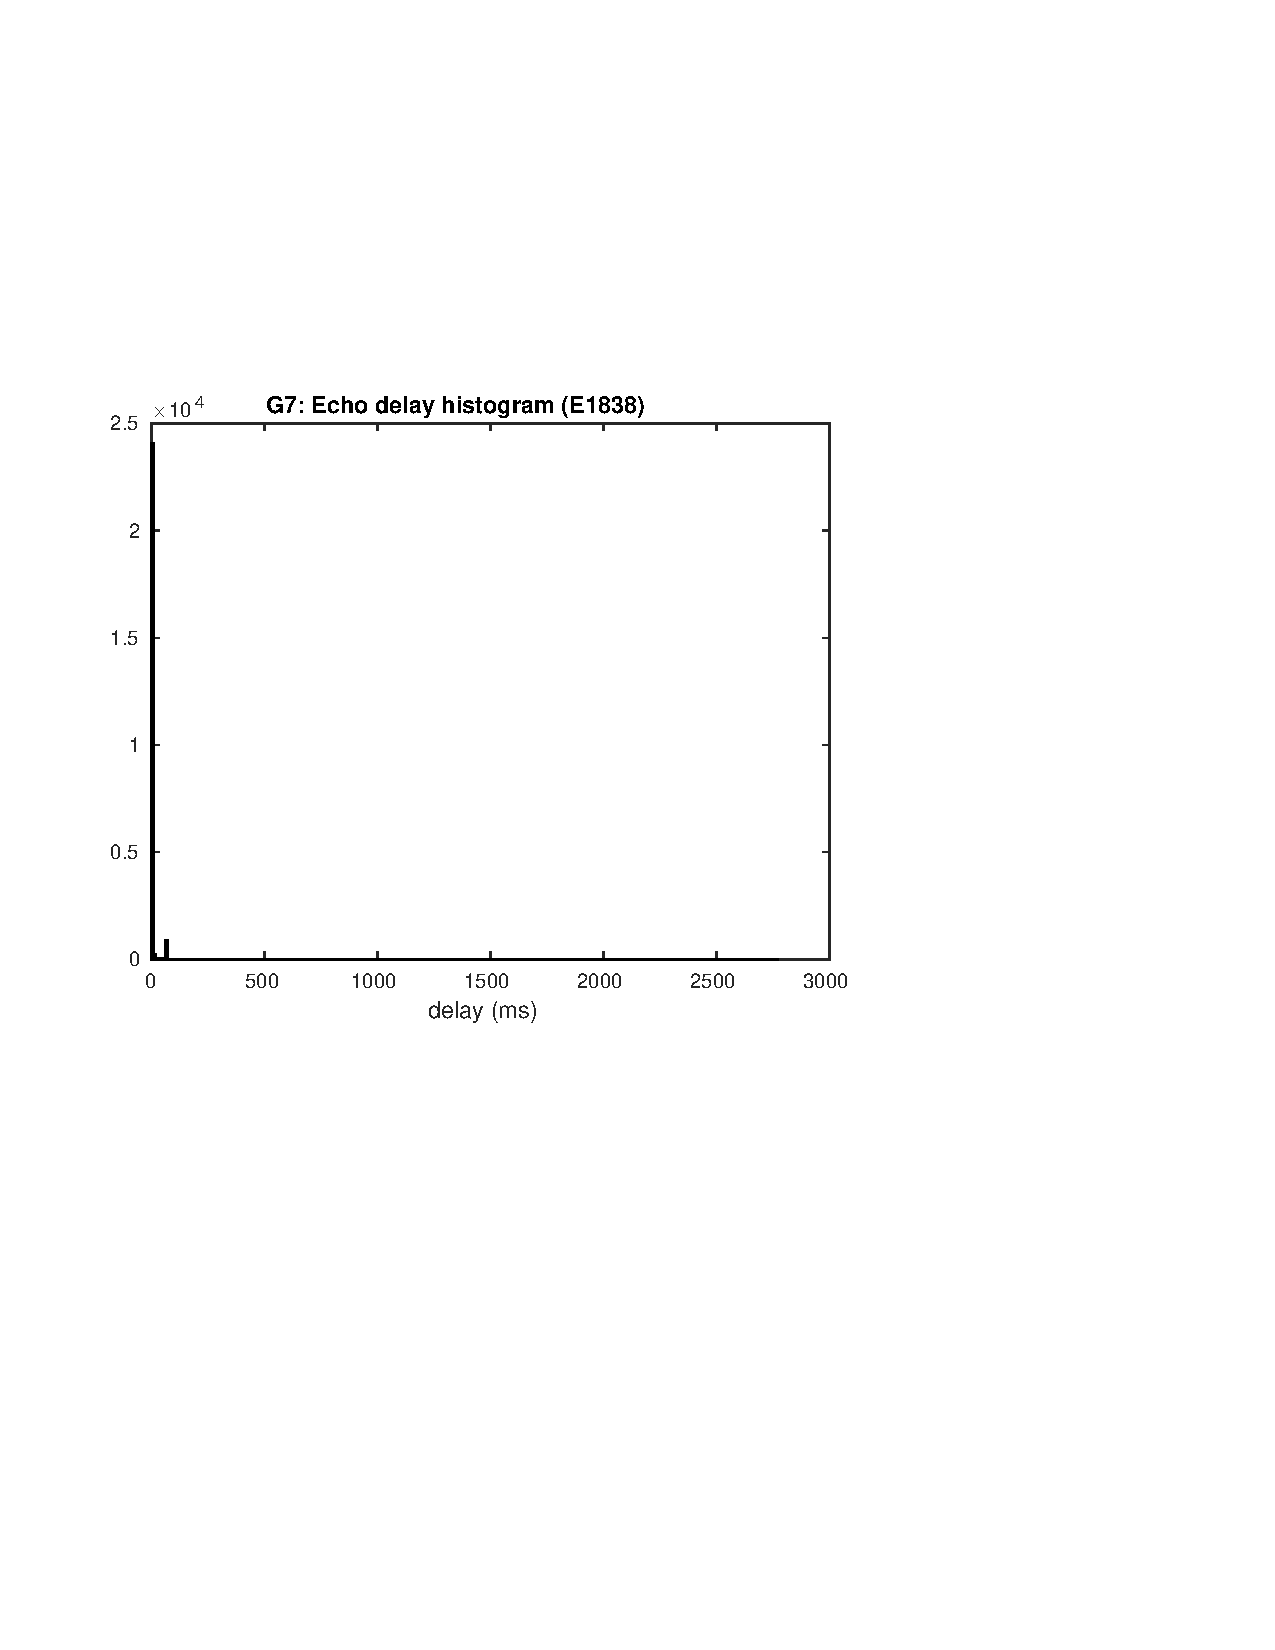
\includegraphics[width=\textwidth]{G7.pdf}
	\end{figure}
	
	\begin{figure}
		\centering
		\includegraphics[width=\textwidth]{G8.pdf}
	\end{figure}
	
	\begin{figure}
		\centering
		\includegraphics[width=\textwidth]{G9.pdf}
	\end{figure}
	
	\begin{figure}
		\centering
		\includegraphics[width=\textwidth]{G10.pdf}
	\end{figure}
	
	\begin{figure}
		\centering
		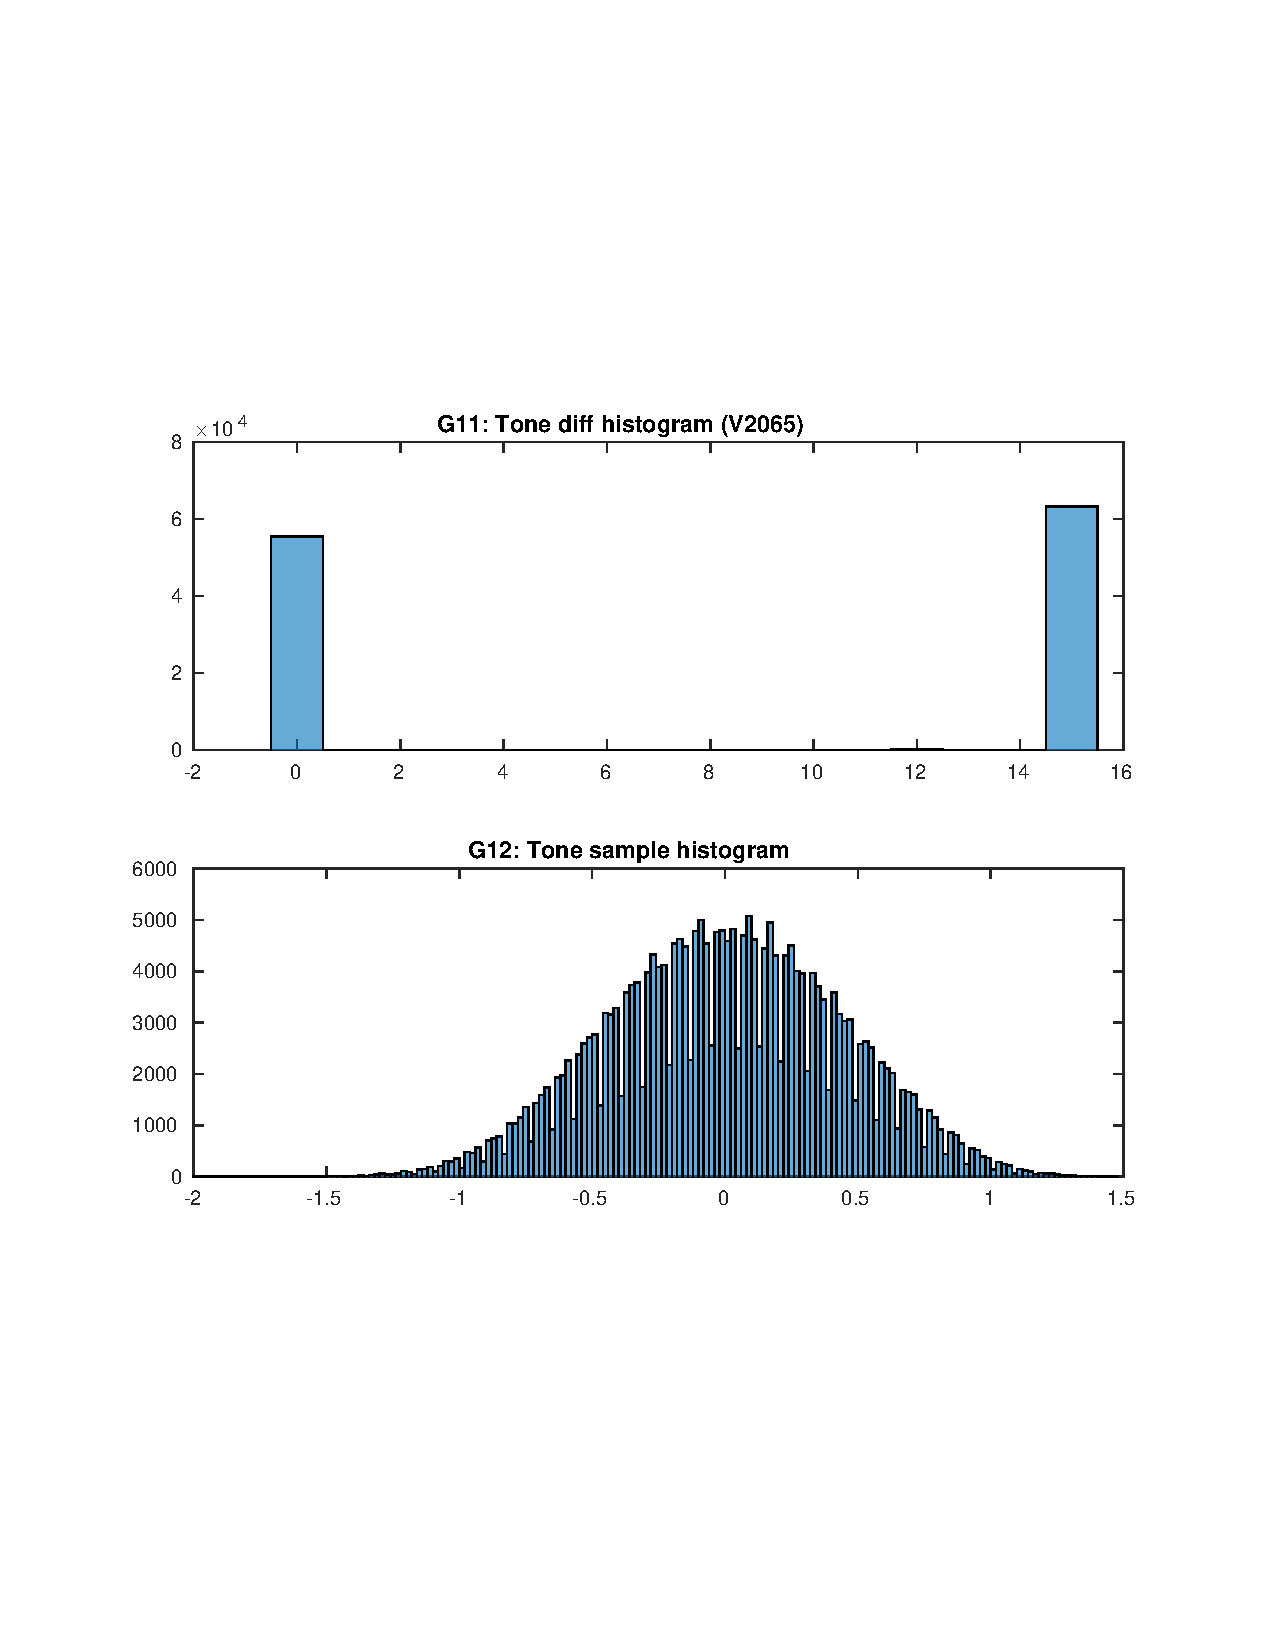
\includegraphics[width=\textwidth]{G11_12.pdf}
	\end{figure}
	
	\begin{figure}
		\centering
		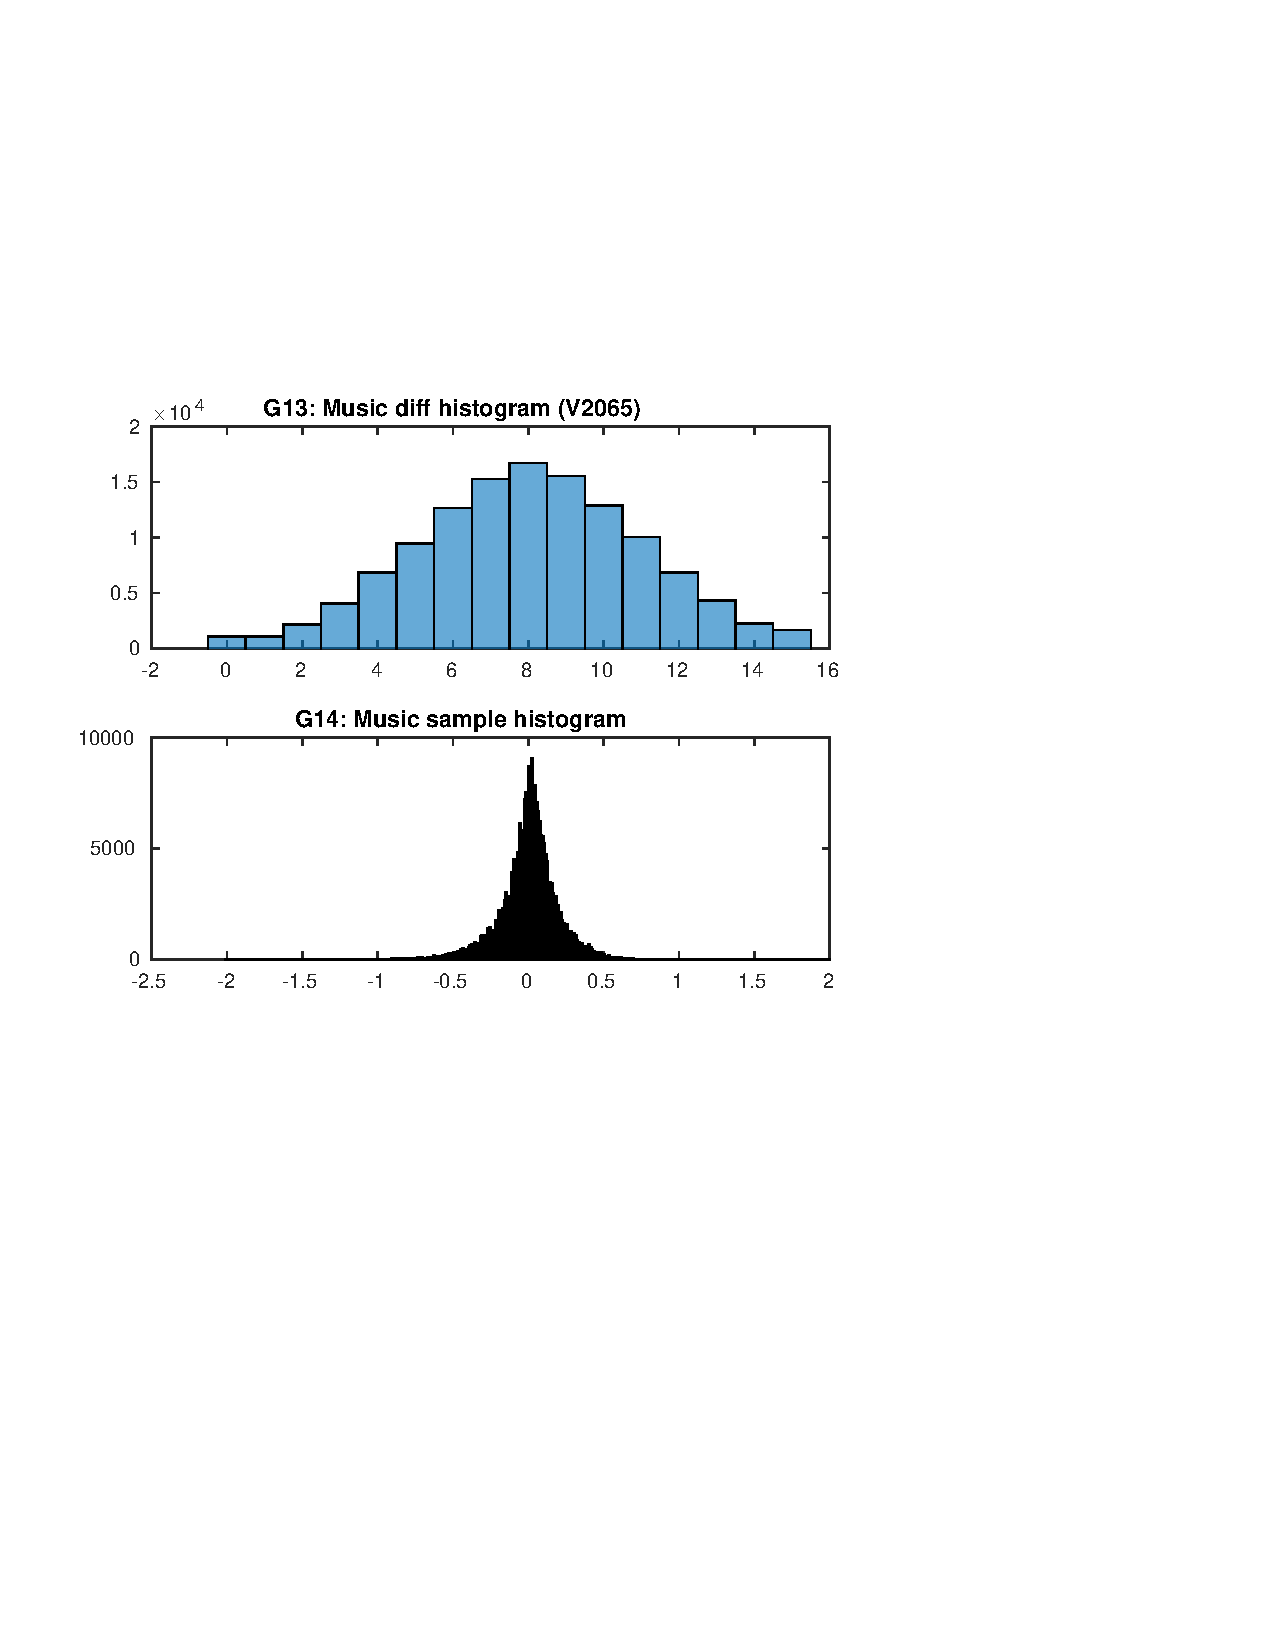
\includegraphics[width=\textwidth]{G13_14.pdf}
	\end{figure}
	
	\begin{figure}
		\centering
		\includegraphics[width=\textwidth]{G15.pdf}
	\end{figure}
	
	\begin{figure}
		\centering
		\includegraphics[width=\textwidth]{G16.pdf}
	\end{figure}
	
	\begin{figure}
		\centering
		\includegraphics[width=\textwidth]{G19.pdf}
	\end{figure}
	
\end{document}
